\section{Metodologia} % Seções são adicionadas para organizar sua apresentação em blocos discretos, todas as seções e subseções são automaticamente exibidas no índice como uma visão geral da apresentação, mas NÃO são exibidas como slides separados.

%----------------------------------------------------------------------------------------

\begin{frame}
    \frametitle{Pipeline}
    \begin{figure}[h]
        \centering
        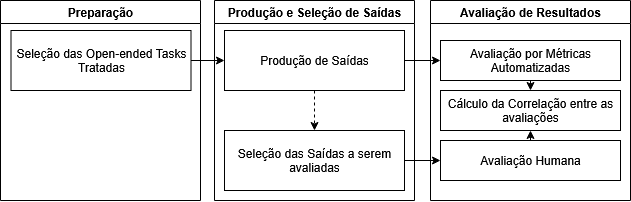
\includegraphics[width=0.95\textwidth]{TCC-Pipeline.png}
        \caption{Pipeline do Trabalho}
        \label{fig:Pipeline}
    \end{figure}
\end{frame}

%----------------------------------------------------------------------------------------

\begin{frame} 
    \only<1>{
        \begin{figure}[h]
            \centering
            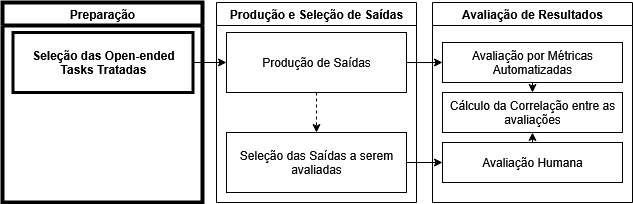
\includegraphics[width=0.95\textwidth]{TCC-Pipeline-tarefas.png}
            \caption{Etapa Atual: Seleção das Tarefas}
        \end{figure}
    }
    \only<2>{
        \frametitle{Tarefas Tratadas}
        \begin{columns}
            \column{0.5\linewidth}
                \begin{figure}
                    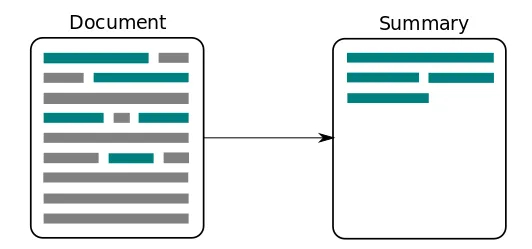
\includegraphics[width=0.8\textwidth]{summ.png}
                    \caption{Sumarização}
                \end{figure}
            \column{0.5\linewidth}
                \begin{figure}
                    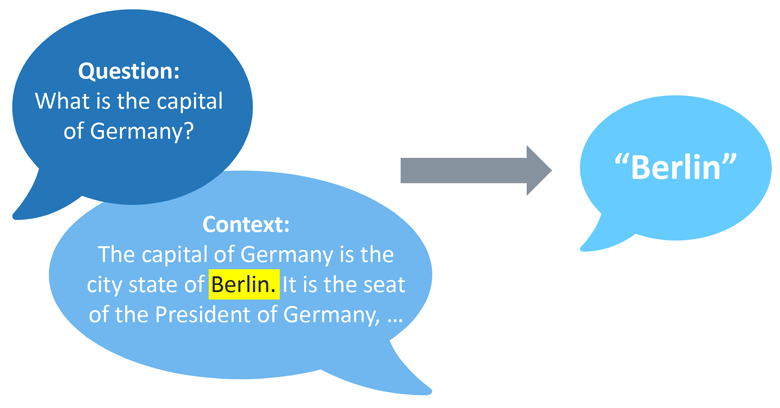
\includegraphics[width=0.8\textwidth]{qamainimage.png}
                    \caption{Question-Answering}
                \end{figure}
        \end{columns}
    }
    \only<3>{
		\frametitle{Abordagens Extrativas x Abstrativas}
		\begin{figure}
			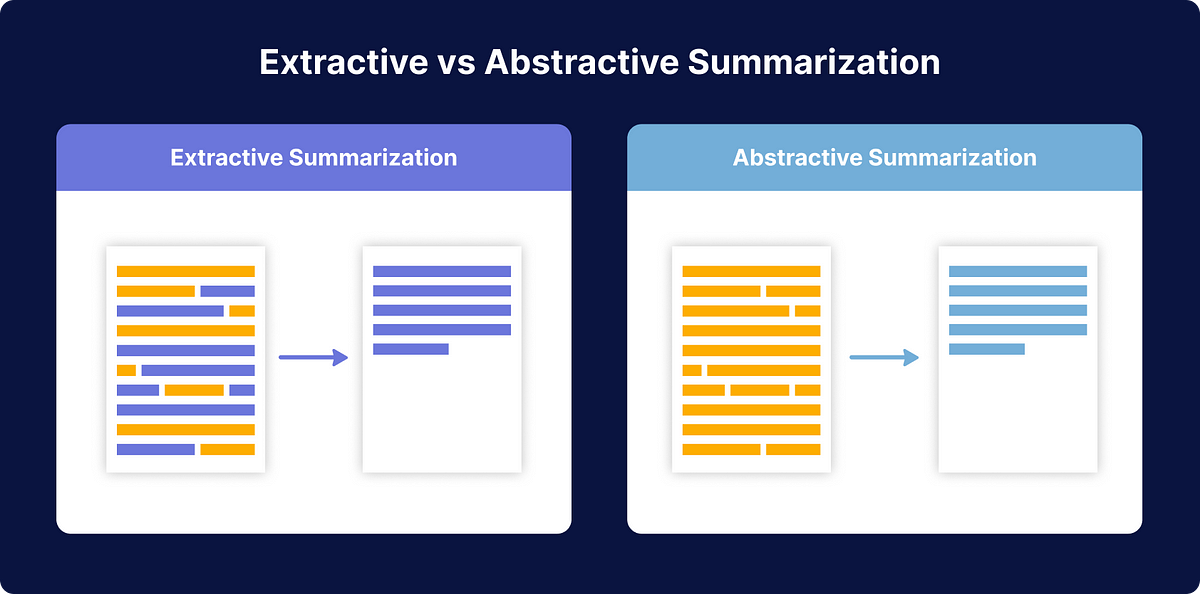
\includegraphics[width=0.8\textwidth]{abs_ext.png}
		\end{figure}
	}
\end{frame}

%----------------------------------------------------------------------------------------

\begin{frame}
    \only<1>{
        \begin{figure}[h]
            \centering
            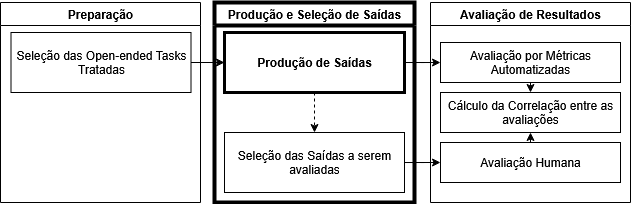
\includegraphics[width=0.95\textwidth]{TCC-Pipeline-producao.png}
            \caption{Etapa Atual: Produção das Saídas}
        \end{figure}
    }
    \only<2>{
        \frametitle{Modelos Utilizados}
        \begin{table}
            \centering
                \begin{tabular}{l c}
                    \hline
                    Tarefa & Modelo\\
                    \hline
                    Sumarização         & PTT5 Summ \\
                    Question-Answering  & Gemma 3   \\
                    \hline
                \end{tabular}
        \end{table}
    }
    \only<3-7>{
        \frametitle{Modelos Utilizados - Sumarização}

        Portuguese T5 for Abstractive Summarization (PTT5 Summ):
        \begin{itemize}[<+(3)->]
            \item Um PTT5 (Carmo et al., 2020) fine-tuned para sumarização
            \item Produzido por Paiola et al. em 2022
            \item Disponibilizado no HuggingFace por Recogna NLP
            \item O modelo escolhido foi fine-tuned sobre o dataset XL-Sum
        \end{itemize}
    }
    \only<8->{
        \frametitle{Modelos Utilizados - Question-Answering}

        Gemma 3:
        \begin{itemize}[<+(8)->]
            \item Uma família de modelos estado da arte leves
            \item Produzido pela Google em 2025
            \item Disponibilizado no HuggingFace pela Google
            \item A versão escolhida foi a it (Instruction Tuned) com 1B de parâmetros. 
        \end{itemize}
    }
\end{frame}

%----------------------------------------------------------------------------------------

\begin{frame}
    \only<1>{
        \frametitle{Datasets Utilizados}
        \begin{table}
            \centering
                \begin{tabular}{l c}
                    \hline
                    Tarefa & Dataset\\
                    \hline
                    Sumarização         & CNN Dailymail Azure Pt    \\
                    Question-Answering  & FairytaleQA Translated Pt \\
                    \hline
                \end{tabular}
        \end{table}
    }
    \only<2-5>{
        \frametitle{Datasets Utilizados - Sumarização}

        CNN Dailymail Azure Pt:
        \begin{itemize}[<+(2)->]
            \item Uma versão traduzida do CNN/DailyMail (Nallapati et al., 2016)
            \item Produzido por Rúben Almeida em 2023
            \item Disponibilizado no HuggingFace pelo autor
        \end{itemize}
    }
    \only<6-9>{
        \frametitle{Datasets Utilizados - Question-Answering}

        FairytaleQA Translated Pt:
        \begin{itemize}[<+(6)->]
            \item Uma versão traduzida do dataset FairyTaleQA (XU et al., 2022)
            \item Produzido por Leite et al. em 2024
            \item Disponibilizado no HuggingFace pelo autor
        \end{itemize}
    }
\end{frame}

%----------------------------------------------------------------------------------------

\begin{frame}
    \only<1>{
        \begin{figure}[h]
            \centering
            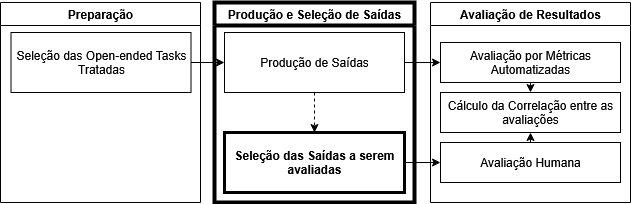
\includegraphics[width=0.95\textwidth]{TCC-Pipeline-selecao.png}
            \caption{Etapa Atual: Seleção das Saídas}
        \end{figure}
    }
    \only<2->{
        \frametitle{Seleção de Saídas}
        \begin{itemize}[<+(1)->]
            \item Amostragem aleatória
            \item 40 saídas por Tarefa
        \end{itemize}
    }
\end{frame}

%----------------------------------------------------------------------------------------

\begin{frame}
    \only<1>{
        \begin{figure}[h]
            \centering
            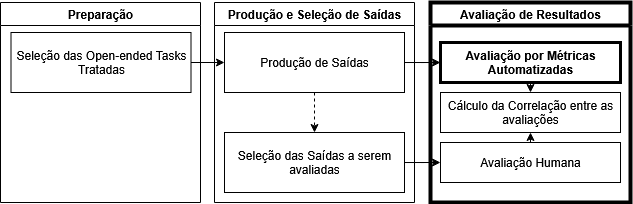
\includegraphics[width=0.95\textwidth]{TCC-Pipeline-metricas.png}
            \caption{Etapa Atual: Avaliação Automatizada}
        \end{figure}
    }
    \only<2>{
        \frametitle{Métricas}
        \begin{table}
            \centering
                \begin{tabular}{l c c c}
                    \hline
                    \textit{Métrica} & \textit{Baseada em} & \textit{Ano Criação} \\
                    \hline
                    \hline
                    BLEU       & $n$-gramas & 2002 \\
                    ROUGE      & $n$-gramas & 2004 \\
                    METEOR     & $n$-gramas & 2005 \\
                    BERTScore  & PLMs       & 2019 \\
                    MoverScore & PLMs       & 2019 \\
                    BARTScore  & PLMs       & 2021 \\
                    \hline
                \end{tabular}
            \caption{Descrição das métricas utilizadas}
        \end{table}
    }
\end{frame}

%----------------------------------------------------------------------------------------

\begin{frame}
    \only<1>{
        \begin{figure}[h]
            \centering
            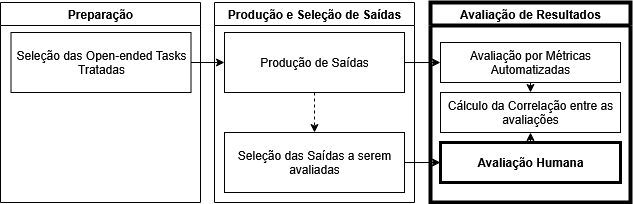
\includegraphics[width=0.95\textwidth]{TCC-Pipeline-humano.png}
            \caption{Etapa Atual: Avaliação Humana}
        \end{figure}
    }
    \only<2-6>{
        \frametitle{Avaliação Humana}
        \begin{itemize}[<+(1)->]
            \item Realizada com 8 pessoas
            \item Dividas em 2 grupos
            \item Cada grupo avaliou 20 saídas de cada tarefa
            \item Totalizando 80 saídas, avaliadas por 4 pessoas cada
            \item As avaliações são realizadas em \textbf{4 dimensões de qualidade}
        \end{itemize}
    }
    \only<7-12>{
        \frametitle{Dimensões de Qualidade}
        \only<7-11>{
            \begin{itemize}[<+(6)->]
                \item Coerência\only<7>{: Qualidade geral do texto}
                \item Consistência\only<8>{: Alinhamento entre a saída e o texto base}
                \item Fluência\only<9>{: Qualidade das frases geradas}
                \item Relevância\only<10>{: Pontos chave selecionados para o texto}
            \end{itemize}
        }
        \only<12>{
            \begin{itemize}
                \item Coerência
                \item Consistência
                \item \textbf{Naturalidade}
                \item Relevância
            \end{itemize}
        }
        
    }
    \only<13->{
        \frametitle{Avaliação Humana}
        \begin{itemize}
            \item Realizada com 8 pessoas
            \item Dividas em 2 grupos
            \item Cada grupo avaliou 20 saídas de cada tarefa
            \item Totalizando 80 saídas, avaliadas por 4 pessoas cada
            \item As avaliações são realizadas em 4 dimensões de qualidade
            \item \textbf{Valor final: a média das avaliações recebidas}
        \end{itemize}
    }
\end{frame}

%----------------------------------------------------------------------------------------

\begin{frame}
    \frametitle{Fomulários}
    \only<1-3>{
        \begin{enumerate}[<+(1)->]
            \item Seleciona seu grupo informado (1 ou 2).
            \item Lê os detalhes de cada saída.
        \end{enumerate}
    }
    \only<4>{
        \begin{table}
            \centering
            \begin{tabular}{l c c c}
                \hline
                \textit{Tarefa} & \textit{Saída} & \textit{Texto/Contexto Base} & \textit{Pergunta}\\
                \hline
                \hline
                Sumarização                 & \checkmark & \checkmark & $X$\\
                \textit{Question-Answering} & \checkmark & \checkmark & \checkmark\\
                \hline
            \end{tabular}
            \caption{Formatação do Formulário.}
            \label{tbl:forms}
        \end{table} 
    }
    \only<5>{
        \begin{enumerate}
            \item Seleciona seu grupo informado (1 ou 2).
            \item Lê os detalhes de cada saída.
            \item Avalia a saída.
        \end{enumerate}
    }
    \only<6>{
        Dimensões de Qualidade:
        \begin{itemize}
            \item Coerência
            \item Consistência
            \item Naturalidade
            \item Relevância
        \end{itemize}
    }
    \only<7>{
        \begin{columns}
            \column{0.5\linewidth}
            \begin{figure}
                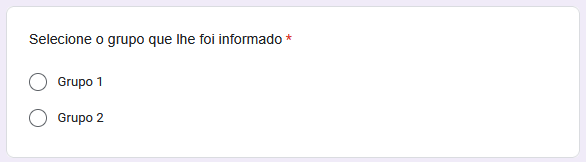
\includegraphics[width=0.8\textwidth]{forms-0.png}
                \caption{Escolha do Grupo}
            \end{figure}
            \begin{figure}
                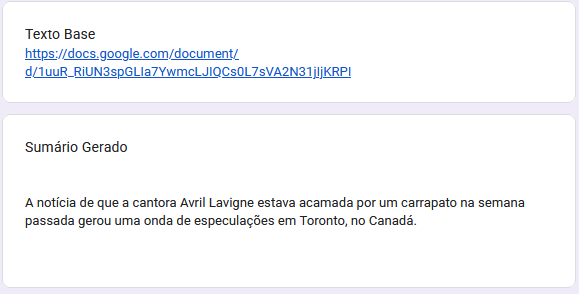
\includegraphics[width=0.8\textwidth]{forms-1.png}
                \caption{Descrição da Saída}
            \end{figure}
            \column{0.5\linewidth}
            \begin{figure}
                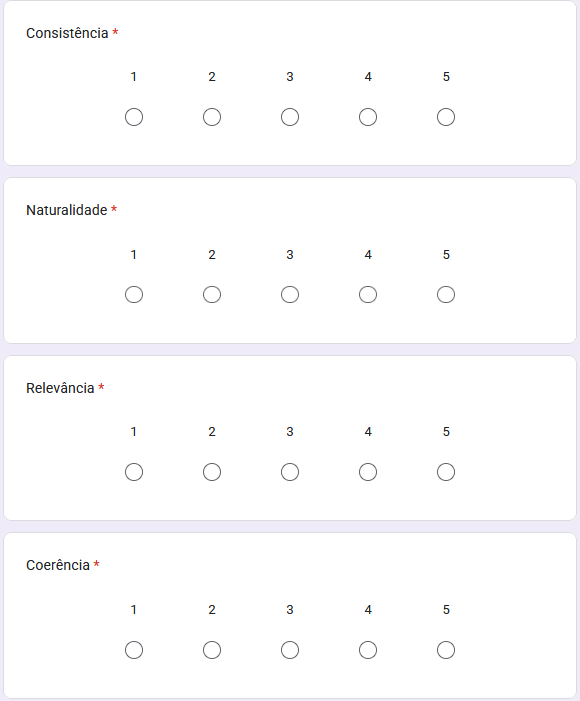
\includegraphics[width=0.8\textwidth]{forms-2.png}
                \caption{Campos de Avaliação}
            \end{figure}
        \end{columns}
    }
\end{frame}

%----------------------------------------------------------------------------------------

\begin{frame}
    \only<2-4>{
        \frametitle{Correlação de Pearson}
    }
    \only<1>{
        \begin{figure}[h]
            \centering
            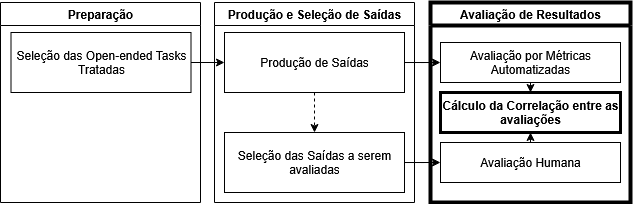
\includegraphics[width=0.95\textwidth]{TCC-Pipeline-correlacao.png}
            \caption{Etapa Atual: Cálculo da Correlação entre Avaliações}
        \end{figure}
    }
    \only<2-3>{
        \begin{itemize}[<+(1)->]
            \item Medida Estatística
            \item Quantificar as relações lineares entre duas variáveis
        \end{itemize}
    }
    \only<4>{
        \begin{table}[htbp]
            \centering
            \begin{tabular}{c l}
                \hline
                Valores de Pearson & Interpretação \\
                \hline
                0.90–1.00 & Muito forte    \\
                0.70–0.89 & Forte          \\
                0.40–0.69 & Moderada       \\
                0.10–0.39 & Fraca          \\
                0.00–0.10 & Negligenciável \\
                \hline
            \end{tabular}
            \caption{Discretização dos valores de Pearson.}
            \label{tbl:pearson}
        \end{table}
    }
    \only<5>{
        \frametitle{Pipeline}
        \begin{figure}[h]
            \centering
            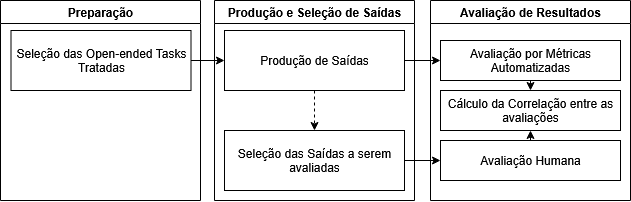
\includegraphics[width=0.95\textwidth]{TCC-Pipeline.png}
            \caption{Pipeline do Trabalho}
        \end{figure}
    }
\end{frame}